\section{Background of the Study}

The world is facing an escalating environmental crisis fueled by the exponential growth of electronic waste (e-waste). In 2019, the global generation of e-waste reached a staggering 53.6 million tons, averaging 7.3 kg per person, and this figure is projected to rise to 74.7 million tons by 2030, almost doubling in just 16 years (Forti et al., 2020). This surge is driven by rapid technological advancements, shorter product life cycles, and increasing consumer demand for the latest gadgets.

Improper disposal of e-waste poses significant threats to both the environment and human health. E-waste contains hazardous substances such as lead, mercury, cadmium, and brominated flame retardants. When e-waste is landfilled or incinerated, these toxins can leach into the soil and water, contaminating ecosystems and posing severe health risks to communities, including neurological damage, respiratory problems, and cancer (Rani et al., 2021 ; Singh et al., 2024). The mishandling of recycling and disposal of e-waste scrap parts poses a high risk of hazardous effects on health and the environment (Rani et al., 2021).

Beyond the environmental and health concerns, the improper management of e-waste represents a significant economic loss. E-waste contains valuable materials such as gold, silver, copper, and platinum, which can be recovered and reused in manufacturing processes. By implementing effective e-waste management systems, we can unlock the potential for resource recovery, reduce our reliance on virgin materials, and create new economic opportunities (Nowakowski et al., 2020).

The academic literature reflects a growing interest in leveraging technology to improve e-waste management. Several studies have explored the application of IoT, AI, and optimization techniques to address various challenges in the e-waste stream.

\begin{itemize}
	\item \textbf{E-waste Identification and Classification:}  Nowakowski & Pamuła (2020) proposed a deep learning-based method for e-waste identification using Convolutional Neural Networks (CNN) and Region-based Convolutional Neural Networks (R-CNN), achieving high classification accuracy (90-96.7\%). Rani et al. (2021) implemented a mobile green e-waste management system using IoT for smart campuses, utilizing the Single Shot Multibox Detector (SSD)Lite-MobileNet-v2 model for e-waste object detection. These studies demonstrate the potential of AI to automate waste sorting and improve the efficiency of recycling processes.
	\item \textbf{Collection Route Optimization:} Nowakowski et al. (2020) combined an artificial intelligence algorithm and a novel vehicle for sustainable e-waste collection. They used the Harmony Search (HS) algorithm for route optimization, which outperformed other algorithms in terms of travel plans, the number of serviced collection points, and profit from collected resources. Aroba et al. (2023) examined the adoption of an intelligent waste collection system in a smart city, using RFID for bin identification, GPS for location tracking, and IoT-enabled sensors for waste level monitoring. These studies highlight the importance of optimizing collection routes to minimize transportation costs and improve the overall efficiency of waste management operations.
	\item \textbf{Smart Waste Management Systems:} Singh et al. (2024) proposed an IoT-enabled Collector Vending Machine (CVM) for e-waste management, allowing customers to dispose of their e-waste and receive a token amount in return. Sharma et al. (2024) focused on essential waste management problems in urban environments, focusing on the escalating electronic waste issue.
\end{itemize}

\noindent However, several limitations and research gaps remain:

\begin{itemize}
	\item \textbf{Dataset Limitations:} Nowakowski & Pamuła (2020) noted that their deep learning model required a larger dataset to improve accuracy and needs validation for other bulky waste categories.
	\item \textbf{Real-World Implementation:} Singh et al. (2024) showed little evidence of practical or real-world implementation and extensive field testing to validate system's effectiveness in diverse conditions
	\item \textbf{Integration Challenges:} There is a need for integrated smart solutions that combine IoT, AI, and optimization techniques to address the complex challenges of e-waste management (Sharma et al., 2024).
	\item \textbf{Predicting Real-World Variables:} Nowakowski et al. (2020) highlight the limited the limitations in predicting real-world variables like equipment size and number, and the novel vehicle design and information system need further real-world testing
\end{itemize}

These gaps highlight the need for further research to develop more robust, scalable, and integrated smart e-waste management solutions that can be effectively deployed in real-world settings.

This study focuses on De La Salle University in the Philippines. This context presents a unique case to study for several reasons: 

As a prominent academic institution located in a highly urbanized area of Metro Manila, the university generates significant amounts of electronic waste (e-waste) due to its reliance on modern technology for educational and administrative purposes. The campus environment provides a controlled setting to test innovative waste management systems while reflecting broader urban challenges faced by developing countries like the Philippines.

The specific issues present in this context include the lack of an efficient e-waste management system within the university, leading to improper disposal practices that contribute to environmental degradation. Additionally, there is no existing mechanism to integrate campus waste management with the city's broader waste disposal infrastructure, which exacerbates inefficiencies and risks. Informal recycling practices also pose potential health and environmental hazards, mirroring challenges seen across urban areas in the country.

Therefore, conducting this study in De La Salle University is crucial to understanding the specific challenges and opportunities for implementing smart IoT-integrated e-waste management solutions in a developing urban environment. The findings of this research can inform the development of targeted strategies and policies to promote sustainable e-waste management and improve the environmental and social well-being of communities in similar contexts.

\section{Prior Studies}

\textbf{Research Gaps Identified}

Numerous previous studies, including those by Pavan et al. (2021) and Nowakowski & Pamuła (2020), use small and specialized datasets that restrict the models' ability to be applied in real-world situations. Additionally, a lot of systems aren't thoroughly field tested, which lowers their dependability and adaptability in a variety of settings.

Due to their high costs, reliance on cutting-edge technologies, and requirement for substantial infrastructure, the solutions suggested in studies such as Sharma et al. (2024) and Huh et al. (2021) have serious scalability problems. These difficulties restrict application in urban and rural environments with limited resources.

A number of studies, such as those by Singh et al. (2024) and Pavan et al. (2021), concentrate on particular waste categories, like dry or e-waste, ignoring the larger requirement for integrated systems that manage bulky or mixed type of waste. This restricts these solutions' usefulness and comprehensiveness.

For intelligent waste management systems, user adoption and behavioral modification continue to be crucial problems. The success of these technologies is undermined by low engagement, which is why studies like Aroba et al. (2023) and Sharma et al. (2024) emphasize the necessity of user-friendly systems and educational campaigns.

There are still problems with hardware performance and reliability, according to Huh et al. (2021) and Nowakowski et al. (2020). Systems frequently depend on particular sensors or algorithms that might perform poorly outside of controlled settings, which would reduce their usefulness in practical applications.

While some studies, like Nowakowski et al. (2020), use algorithms like Harmony Search to optimize routes, they frequently overlook dynamic variables that are essential for effective logistics, such as real-time traffic or fluctuating waste volumes. \newline 

\noindent \textbf{Proposal to Address the Gaps}

This proposal will create a large, diverse dataset covering different waste categories (such as dry, e-waste, and bulky items) under various environmental conditions in order to overcome the limitations of small and specialized datasets. Accuracy of real-world systems and model training will both benefit from this.

Using a modular architecture, the suggested system will integrate AI and IoT technologies while permitting scalability. Lightweight sensors and cloud-based data processing are examples of affordable alternatives that can be used to customize features for regions with limited resources.

This system will have dynamic classification capabilities using cutting-edge machine learning models, in contrast to current solutions that concentrate on particular waste types. This will make it possible to handle bulky and mixed waste effectively, providing a more comprehensive approach to waste management.

The addition of redundant sensors and algorithms will improve the system's dependability. Models will be adjusted to different environments by machine learning techniques like transfer learning, guaranteeing consistent performance even under trying circumstances.

To increase the effectiveness of waste collection, real-time traffic data and adaptive route optimization algorithms will be combined. Adjustments based on bin status, traffic, and other environmental constraints will be possible thanks to this dynamic approach.

To assess the system's operational effectiveness, user acceptability, and scalability, pilot projects will be carried out in a variety of urban and rural locations. Iterative improvements will be made based on input from these pilots to make sure the system satisfies practical needs.

By addressing these gaps, the suggested system seeks to provide a thorough, flexible, and easy-to-use waste management solution that will greatly aid in the development of sustainable urban and rural areas.

\section{Problem Statement}

Effective waste management is a critical component of sustainable urban and rural development. However, existing systems face significant challenges, including inefficiencies in classification and collection, high costs, low public engagement, and inadequate scalability, as outlined below.


\begin{enumerate}
	\item PS1: The Ideal Scenario
	\begin{itemize}
		\item Communities should have access to an efficient, intelligent waste management system that accurately classifies, collects, and processes various types of waste.
		\item Waste disposal should be environmentally sustainable, cost-effective, and scalable, benefiting both urban and rural areas.
		\item Public engagement in waste segregation and recycling should be seamless, supported by user-friendly technology and educational initiatives.
	\end{itemize}
	
	\item PS2:  The Reality of the Situation
	\begin{itemize}
			\item Existing waste management solutions rely on small, specialized datasets, limiting their ability to perform effectively in real-world environments.
			\item Many systems are expensive, technologically complex, and require substantial infrastructure, making them unsuitable for regions with limited resources.
			\item Current solutions often focus on specific waste categories (e.g., dry or e-waste), ignoring the need for integrated systems that handle mixed or bulky waste.
			\item User participation remains low due to a lack of incentives, awareness, and accessible platforms for engagement.
			\item Waste collection logistics are inefficient due to static routing methods that fail to account for real-time traffic conditions and fluctuating waste volumes.
	\end{itemize}
	
	\item PS3:  The Consequences for the Audience		
	\begin{itemize}
			\item Inefficient waste management leads to environmental degradation, increased pollution, and overburdened landfills.
			\item High operational costs and resource wastage continue to strain local governments and waste management authorities.
			\item Low public participation in waste segregation results in ineffective recycling efforts and excessive landfill use.
			\item Inconsistent or delayed waste collection services contribute to unsanitary conditions, negatively affecting public health.
			\item Without scalable and adaptive waste management solutions, sustainable development goals remain unattainable, particularly in resource-limited communities.
	\end{itemize}

\end{enumerate}

This proposal introduces a smart waste management system that integrates AI and IoT technologies to optimize waste classification, segregation, and collection. Using machine learning, the AI model will identify and classify different types of waste with high accuracy, enabling automated segregation and reducing human error. Real-time data processing will enhance adaptability, allowing the system to adjust based on varying waste compositions and environmental conditions. Additionally, a user-friendly platform with gamification elements will encourage community participation in waste segregation. By improving efficiency, scalability, and engagement, this solution aims to create a more sustainable and accessible waste management system.

\section{Objectives and Deliverables}

\subsection{General Objective (GO)}
\Copy{GO}{GO: To develop an intelligent waste management system that integrates deep learning and loT technologies for accurate classification and optimized collection of e-waste, improving recycling efficiency and sustainability.};

\subsection{Specific Objectives (SOs)}

\begin{itemize}
	\item \Copy{SO1}{SO1: To Create an expanded dataset which includes a wider but manageable selection of e-waste categories including small electronics and large appliances and batteries and circuit boards.  }
	
	\item \Copy{SO2}{SO2: To Design a system that can identify and differentiate e-waste and normal waste along with types in a single image or detection process.}
	
	\item \Copy{SO3}{SO3: To create a deep learning model  (e.g., CNN, Faster R-CNN)  developed through training and optimization for e-waste category classification while achieving at least 90\% accuracy on test dataset assessment. }
	
	\item \Copy{SO4}{SO4: To Integrate IoT for better monitoring (e.g. use of sensors, mobile app) to track e-waste disposal and automate collection scheduling based on bin capacity and waste type.}
	
\end{itemize}


\subsection{Expected Deliverables}

TableTables~\ref{tab:expected_deliverables_1} and \ref{tab:expected_deliverables_2} shows the outputs, products, results, achievements, gains, realizations, and/or
yields of the \documentType. 

\begin{table}[!htbp]
	\footnotesize
	\caption{Expected Deliverables per Objective (Part 1)}
    \label{tab:expected_deliverables_1}
    \centering
    \begin{tabular}{p{0.2\textwidth}|p{0.7\textwidth}}
        \hline 
        \hline 
        \textbf{Objectives} & \textbf{Expected Deliverables} \\ 
        \hline 
        \Paste{GO} &  
		\begin{enumerate}
			\item \textbf{Expanded E-Waste Dataset:} \begin{itemize}
				\item A comprehensive dataset in CSV or JSON format with at least 100 entries covering key e-waste categories (small electronics, appliances, batteries, circuit boards). 
				\item Detailed fields on material composition, weight ranges, hazardous components, and recycling methods. 
				\end{itemize}
			\item \textbf{Trained MobileNet Model:}  \begin{itemize}
				\item A deep learning-based image recognition model capable of accurately classifying e-waste and normal waste with 90\%+ accuracy.
			\end{itemize}
			\item \textbf{Real-Time Classification System:}  \begin{itemize}
				\item A functional system with a user interface for uploading images and real-time waste classification. 
				\item Outputs include item classification (e-waste or normal waste) and detailed type categorization with confidence scores. 
				\item Smart bins with sensors for real-time tracking of bin capacity, waste type identification, and automated collection scheduling. 
				\item A cloud-based dashboard for monitoring bin status and collection history, integrated with a mobile app for waste management personnel and users. 
			\end{itemize}
			\item \textbf{Optimized Collection Process:} \begin{itemize}
				\item Automated collection scheduling based on bin capacity and waste type, optimizing collection routes and reducing operational inefficiencies. 
			\end{itemize}
			\item \textbf{Sustainability Gains:}  \begin{itemize}
				\item Improved recycling efficiency by enhancing e-waste classification and automating the collection process. 
				\item Reduced environmental impact through better management of e-waste disposal. 
			\end{itemize}
		\end{enumerate} \\ \hline

		\Paste{SO1} & 
		\begin{enumerate}
		\item The dataset will include detailed fields such as the specific subcategory of items (e.g., smartphones, refrigerators, lithium-ion batteries, PCBs), material composition (e.g., plastics, metals, rare earth elements), typical weight ranges (e.g., 0.1–0.5 kg), hazardous components (e.g., lead, mercury), and standard recycling methods (e.g., shredding, smelting).
		\item It will be provided in CSV or JSON format and will include metadata summarizing the total entries and data sources. 
		\item The dataset will feature at least 100 entries distributed across the four categories, ensuring comprehensive coverage of key e-waste types.		
		\end{enumerate} 
        \\ \hline  
    \end{tabular}
\end{table}

\begin{table}[!htbp]
    \footnotesize
    \caption{Expected Deliverables per Objective (Part 2)}
    \label{tab:expected_deliverables_2}
    \centering
    \begin{tabular}{p{0.2\textwidth}|p{0.7\textwidth}}
        \hline 
        \hline 
        \textbf{Objectives} & \textbf{Expected Deliverables} \\ 
        \hline 

		\Paste{SO2} & 
		\begin{enumerate}
		\item The system will use a machine learning-based image recognition model (MobileNet), trained on a diverse dataset of labeled images covering various types of e-waste (e.g., circuit boards, small electronics, batteries) and normal waste (e.g., paper, plastic, organic waste). 
		\item Trained model, a user interface for uploading images, and real-time detection capabilities. 
		\item Outputs will specify whether the detected item is e-waste or normal waste and, if e-waste, classify it into predefined types. 
		\item The system will also generate confidence scores for each classification and provide a summary report of the detected items. It will be deployable via a desktop application or embedded system for on-site waste sorting.
		\end{enumerate} \\ \hline
		
		\Paste{SO3} & 
		\begin{enumerate}
		\item The model will be trained using transfer learning on MobileNet's pre-trained weights, followed by fine-tuning to adapt it to the specific e-waste categories. Hyperparameters like learning rate, batch size, and number of epochs will be optimized, and techniques such as dropout will be applied to prevent overfitting. 
		\item The performance of the model will be evaluated using metrics like accuracy, precision, recall, and F1-score, with a focus on achieving at least 90\% accuracy on unseen test data. 
		\item Trained MobileNet model in a deployment-ready format (e.g., TensorFlow Lite or ONNX) for efficient real-time classification, along with detailed documentation of the training process, optimization techniques, and performance evaluation results.
		\end{enumerate} \\ \hline
					
		\Paste{SO4} & 
		\begin{enumerate}
		\item The system integrates smart sensors and a mobile application to monitor bin capacity and classify waste types in real time. Smart bins will be equipped with ultrasonic sensors to measure bin capacity, load cells for weight measurement, and RFID or image sensors for identifying the type of waste (e.g., small electronics, batteries). These sensors will be connected via Wi-Fi or LoRa modules to transmit data to the cloud. 
		\item The system will feature a cloud-based dashboard displaying real-time bin status, waste type, and collection history, while a mobile app will allow both users and waste management personnel to view bin locations, capacity, and collection schedules. Automated collection scheduling will be triggered when bins reach predefined thresholds (e.g., 90\% full) and will prioritize bins based on factors such as capacity, location, and waste type to optimize collection routes.
		\end{enumerate} \\ \hline

    \end{tabular}
\end{table}

\section{Significance of the Study}

\subsection{Technical Benefit}

The technical innovations in this study contribute to improving the accuracy, efficiency, and scalability of e-waste management systems. It introduces a Smart IoT-Integrated Waste Management System that uses cloud computing to enhance e-waste classification and collection efficiency. The integration of IoT-enabled smart bins equipped with Raspberry Pi, cameras, and sensors enables automatic detection, classification, and monitoring of waste levels. Moreover, by utilizing a MobileNet-based deep learning model, the system ensures real-time and accurate classification of e-waste items, reducing errors commonly found in traditional waste segregation methods.  These bins communicate with a cloud-based infrastructure, allowing seamless data processing and real-time updates for waste collection scheduling. This research enhances automation in waste management, reducing manual labor while improving overall system efficiency. By optimizing waste collection schedules and minimizing unnecessary pickups, the system contributes to lower operational costs, improved recycling processes, and a more scalable approach to modern e-waste management.

\subsection{Social Impact}

The implementation of a smart e-waste management system can contribute to  improving public health, promoting environmental awareness, and enhancing waste management practices. E-waste contains several hazardous heavy metals and chemicals, with proper classification and disposal of e-waste of the proposed system, it can help reduce toxic exposure and prevent toxic substances from contaminating living spaces, reducing relatively the health risks associated with prolonged exposure. Furthermore, the system encourages public participation in responsible e-waste disposal through its mobile application, which provides users with real-time waste level alerts and disposal recommendations. By increasing awareness and fostering more responsible waste habits, the project promotes a cleaner and more sustainable society. Additionally, optimized waste collection reduces the accumulation of improperly disposed e-waste in public areas, contributing to improved urban sanitation and overall quality of life.

\subsection{Environmental Welfare}

This study will contribute to reducing pollution and promoting sustainable waste management practices. With effective classification and proper handling or disposal of e-waste, the proposed system can reduce harmful pollutants commonly found in e-waste, such as lead, mercury, and cadmium, preventing these materials from contaminating soil and water. Moreover, the optimized waste collection scheduling also helps lower the carbon footprint by minimizing fuel consumption and emissions from waste transport vehicles. Through these combined efforts, the study promotes a tech-driven, eco-friendly approach to waste management, aligning with global sustainability goals and ensuring long-term environmental protection.

\section{Assumptions, Scope, and Delimitations}

%Bulletize your assumptions in one group, and then bulletize the scope in another, and do the same for your delimitations. The assumptions to put here are those major facts or statements that are \textit{key} for your proposed solution to work. Scope refers to the space(s) for the operation of your proposed solution, whereas delimitations are the limits of the operation of your proposed solution.

\subsection{Assumptions}

\begin{enumerate}
\item Technical Infrastructure
	\begin{itemize}
		\item The designed system needs constant internet access to maintain real-time data exchange between IoT devices and cloud servers.
		\item The system integration between deep learning models and IoT devices and cloud-based infrastructure operates smoothly to provide stable data transfer during real-time processing while avoiding significant technical issues.
		\item The system will have access to a steady electricity supply at bin locations to enable system operation.
		\item Raspberry Pi hardware can adequately process image classification tasks using the MobileNet model.
	\end{itemize}

\item Data Accuracy
	\begin{itemize}
		\item The datasets from sources such as ImageNet, COCO, and the custom dataset are comprehensive, accurately labeled, and reflective of real-world e-waste and normal waste conditions.
	\end{itemize}

\item Model Performance
	\begin{itemize}
		\item The pre-trained MobileNet model, once fine-tuned on the dataset, will achieve at least 90\% accuracy in classifying various e-waste categories and differentiating them from normal waste.
	\end{itemize}

\item Sensor Reliability
	\begin{itemize}
		\item The IoT sensors integrated into the smart bins (e.g., ultrasonic sensors for bin capacity) will operate reliably under a range of environmental conditions, providing accurate and consistent data.
		\item Images captured by bin cameras will have sufficient resolution for accurate waste classification.
	\end{itemize}

\item User Interaction
	\begin{itemize}
		\item It is assumed that waste management personnel and end-users possess technological literacy that enables them to interact with the system as intended, providing consistent data input and adhering to proper waste segregation practices, which is critical for the system’s real-time functionality.
	\end{itemize}

\item Operating Environment
	\begin{itemize}
		\item Environmental conditions, together with power and network breakdowns, will not significantly affect system performance.
		\item System maintenance is performed routinely and at normal intervals.
	\end{itemize}
\end{enumerate}

\subsection{Scope}
The scope of this study encompasses the development and implementation of an intelligent e-waste management system that utilizes IoT and deep learning technologies. The system is designed to classify and optimize the collection of electronic waste, ensuring efficient and accurate waste segregation. Key aspects of the study include:

\begin{enumerate}
    \item \textbf{Waste Classification and Collection}
    \begin{enumerate}
        \item The system focuses on identifying and classifying electronic waste using deep learning models.
        \item Waste images are captured using a Raspberry Pi camera and processed through a MobileNet-based classification model.
        \item Smart bins are integrated with IoT sensors to monitor waste levels and optimize collection schedules.
    \end{enumerate}
	
	\item \textbf{Machine Learning Model Implementation}
    \begin{enumerate}
        \item The study employs a pre-trained MobileNet model, fine-tuned for e-waste classification.
        \item The dataset for model training is sourced from ImageNet, COCO, and a custom dataset.
        \item The model aims to achieve at least 90\% accuracy in distinguishing e-waste from general waste.
    \end{enumerate}

    \item \textbf{IoT and Cloud Infrastructure}
    \begin{enumerate}
        \item The system integrates IoT sensors, including ultrasonic sensors, for bin capacity monitoring.
        \item Data exchange occurs in real-time between IoT devices and cloud-based servers.
        \item A stable internet connection and continuous power supply are assumed for uninterrupted system operation.
    \end{enumerate}

    \item \textbf{User Interaction and System Monitoring}
    \begin{enumerate}
        \item The system is intended for use by waste management personnel with adequate technological literacy.
        \item A mobile application provides real-time alerts and bin status monitoring for administrators.
        \item The app does not include in-depth analytics dashboards or public user reporting features.
    \end{enumerate}

    \item \textbf{Operating Environment and Maintenance}
    \begin{enumerate}
        \item The system is designed to function under standard environmental conditions with minimal disruption due to network or power failures.
        \item Regular maintenance is assumed to ensure optimal performance of IoT sensors and deep learning models.
    \end{enumerate}
\end{enumerate}

\subsection{Delimitations}
\begin{enumerate}
	\item Focus on E-Waste Management
		\begin{itemize}
			\item This study is limited to the classification, collection, and optimization of electronic waste (e-waste). Other types of general waste (e.g., biodegradable, non-biodegradable, hazardous waste) are not included in the dataset or classification model.
		\end{itemize}

	\item Dataset Sources for Training
		\begin{itemize}
			\item The training dataset is sourced from ImageNet, COCO, and a custom dataset. Additional public datasets or synthetically generated data are not included in this study.
		\end{itemize}

	\item IoT Hardware and Sensor Limitations
		\begin{itemize}
			\item The system is designed for use with Raspberry Pi and its connected camera module. Other hardware platforms like Jetson Nano, Arduino, or industrial-grade AI processors are not included.
			\item The trash level sensors track only bin capacity; other environmental sensors (e.g., temperature, humidity, gas sensors for hazardous waste, measure weight, or toxicity of e-waste items)are not integrated.
		\end{itemize}

	\item Machine Learning Model and Performance Constraints
		\begin{itemize}
			\item The system exclusively uses MobileNet, meaning other deep learning architectures (e.g., EfficientNet, ResNet, or custom CNNs) are not benchmarked.
		\end{itemize}

	\item Mobile App Functionality Constraints
		\begin{itemize}
			\item The app is used for alert notifications and bin status monitoring, but it does not include detailed analytics dashboards for in-depth waste trend visualization.
			\item The mobile app is used by administrators; it does not provide a public user interface for individuals to report or track waste disposal.
		\end{itemize}
		


\end{enumerate}

\section{Description and Methodology of the \documentType}

%A purpose of the description here is to re-steer/remind the panelist/reader again by tersely describing what your thesis is about (i.e. the problem and the main goal you want to achieve) in another way without sounding repetitive. 

%Your methodology is your means of achieving your stated objectives. What you put here is the summary of your methodology chapter.
\begin{figure}[!htbp]
	\centering
		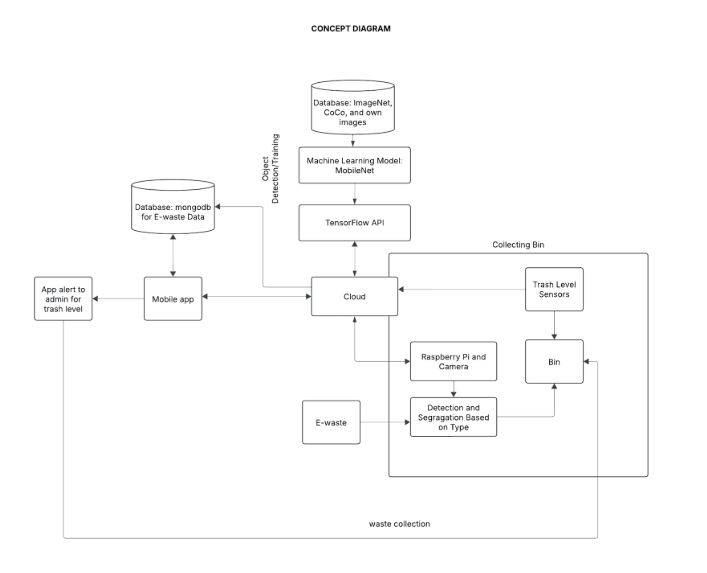
\includegraphics[width=0.5\textwidth]{Conceptual_Diagram.png}
	\caption{Proposed Conceptual Diagram}
	\label{fig:Description and Methodology}
\end{figure}

The concept diagram illustrates the research's system architecture, focusing on the backend operations of the collecting bin. At its core, the system leverages object detection and classification using a database of images, including ImageNet, CoCo, and custom datasets. MobileNet serves as the machine learning model, with TensorFlow as the API to facilitate the training process. These components are integrated into a cloud-based infrastructure, enabling seamless communication between the collecting bin and other system elements. 

The collecting bin employs IoT features, with a Raspberry Pi and camera executing the trained MobileNet model to detect and classify e-waste. Once classified, the waste is segregated and directed to the appropriate bin. Each bin is equipped with trash level sensors that monitor capacity. When the trash level reaches a predefined threshold, the sensors send a signal to the cloud, triggering notifications to the mobile app used by administrators or designated personnel.

The mobile app, connected to a MongoDB database, provides real-time trash data analytics, including bin status and alert management. Upon receiving an alert, administrators can efficiently schedule waste collection. This system ensures timely waste segregation and disposal, streamlining e-waste management and promoting sustainability. 

\textbf{Data Collection}

The data collection process for the e-waste management system is divided into backend and frontend operations to ensure efficient training, classification, and monitoring of waste disposal. 

\newline \noindent Backend Data Collection (Training and Processing)
\begin{enumerate}
	\item Image Dataset Compilation \par
The object detection and classification system leverages multiple datasets to train the MobileNet model effectively. These datasets include: 
	\begin{itemize}
		\item \textbf{ImageNet:} Provides a large-scale dataset of diverse object images for broad recognition capabilities (minimum 1000 images).
		\item \textbf{CoCo (Common Objects in Context):} Offers contextual understanding of e-waste items within various environments (minimum 1000 images).
		\item \textbf{Custom Dataset:} Includes curated images of specific e-waste items such as discarded mobile phones, circuit boards, batteries, and other electronic components (minimum 2000 images for better model adaptation to domain-specific waste).
	\end{itemize} 

These datasets undergo preprocessing, annotation, and augmentation to enhance classification accuracy. The training phase uses \textbf{TensorFlow APIs} for model optimization, ensuring high-performance detection. \newline
	
	\item Model Deployment and Cloud Integration 
	
	Once trained, the MobileNet model is deployed within a \textbf{cloud-based infrastructure} for real-time processing. The backend system performs:
	
	\begin{itemize}
		\item \textbf{Classification Processing:} Running inference on new waste images captured by the IoT-enabled bin.
		\item \textbf{Data Storage:} Storing classification results, confidence scores, and waste images in a \textbf{MongoDB database.}
		\item \textbf{Performance Monitoring:} Continuously evaluating classification accuracy and retraining the model as needed based on new data.
	\end{itemize}
\end{enumerate}

\noindent Frontend Data Collection (IoT Bins and Analytics)
\begin{enumerate}
	\item Data Collection via IoT-Enabled Collecting Bin \par

	The physical collecting bin integrates IoT components to classify and monitor waste disposal. Key features include: \begin{itemize}
	
		\item A \textbf{Raspberry Pi with a camera module} capturing images of disposed e-waste.
		\item Real-time classification of e-waste items using the deployed MobileNet model.
		\item \text{Data logging}, which records: \begin{enumerate}
			\item Timestamp of waste disposal
			\item Classified waste type
			\item Confidence score of classification
			\item Bin ID (location identifier) 
		\end{enumerate}
	\end{itemize}
	\item Trash Level Monitoring and Alerts

	 Each bin is fitted with \textbf{sensors} to track waste accumulation. The sensors provide: \begin{itemize}
		
		\item \textbf{Real-time bin capacity data}, updated at regular intervals.
		\item \textbf{Threshold alerts}, sent to the cloud system when a bin reaches its maximum capacity.
		\item \textbf{Historical disposal trends}, aiding in predictive waste management and optimized collection scheduling.
	\end{itemize}
\end{enumerate}

\textbf{Data Analysis} 
	
	The data collected from the backend machine learning model and the frontend IoT-enabled waste bins undergoes systematic analysis to enhance the efficiency of e-waste classification, optimize collection schedules, and assess the environmental impact of the system. 

\begin{enumerate}
	\item Machine Learning Model Performance Evaluation \\
To ensure the MobileNet classification model performs optimally, backend data is analyzed using:
	\begin{itemize}
		\item \textbf{Precision, Recall, and F1 Score:} Evaluate classification accuracy by measuring false positives and false negatives.
		\item \textbf{Confusion Matrix:} Visualizes misclassified e-waste items, aiding in model improvement.
		\item \textbf{Cross-Validation:} Splits the dataset into training and validation sets to assess performance across different data samples.
		\item \textbf{Retraining Frequency:} Regularly updates the dataset and retrains the model based on misclassified images to enhance accuracy.
	\end{itemize}
	\item Waste Classification Trends and Prediction \\
Frontend data collected from IoT bins helps identify e-waste disposal trends. Analytical methods include:
	\begin{itemize}
		\item \textbf{Classification Frequency Analysis:} Uses statistical aggregation to determine the most frequently disposed waste items.
		\item \textbf{Time-Series Analysis:} Forecasts future disposal rates using models such as ARIMA (AutoRegressive Integrated Moving Average).
		\item \textbf{Pattern Recognition:} Employs clustering algorithms,  K-Means to detect disposal trends and recommend bin placement adjustments.
	\end{itemize}
	\item Bin Capacity and Collection Optimization \\
Sensor data from waste bins is analyzed to optimize collection schedules such as:
	\begin{itemize}
		\item \textbf{Predictive Maintenance:} Implements machine learning algorithms to predict when bins will be full based on historical disposal rates.
	\end{itemize}
\end{enumerate}

\ifFinished
\else

\section{Estimated Work Schedule and Budget}

%The estimated work schedule can be represented as a Gantt Chart or a combination of Project Network Diagram, Work Breakdown Structure, and Critical Path.  The budget can be made into a Bill of Materials, financial plan, or if your \documentType \ is funded and part of larger project, the cost, and date for reaching each milestone and/or deliverable for your part of the project.

%For ECE Department undergraduate theses, the individual Gantt Chart or Work Breakdown Schedule and Bill of Materials will be included in this section and be removed in the final document.

%\graytx{\blindtext}

\subsection{Gantt Chart}
\FloatBarrier 
\begin{figure}[!htbp]
	\centering
		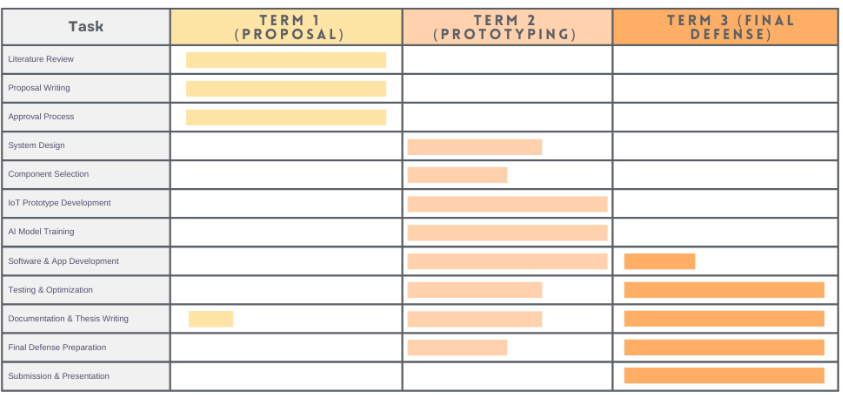
\includegraphics[width=0.5\textwidth]{Gantt_chart.png}
	\caption{Gantt Chart.}
	\label{fig:exampletc}
\end{figure}

\clearpage  % Forces everything before moving on

\subsection{Estimated Budget}

\FloatBarrier  % Ensures the Gantt chart is placed before proceeding

\begin{table}[!htbp]
    \centering
    \caption{List of Components and Costs}
    \label{tab:ComponentCosts}
    \scriptsize
    \renewcommand{\arraystretch}{1.3} % Adjusts row height
    \resizebox{\textwidth}{!}{ % Resizes table to fit page width
        \begin{tabular}{|p{0.2\textwidth}|p{0.3\textwidth}|p{0.1\textwidth}|p{0.15\textwidth}|p{0.15\textwidth}|}
            \hline
            \rowcolor[HTML]{D9D9D9} 
            \textbf{Item} & \textbf{Description} & \textbf{Quantity} & \textbf{Unit Cost} & \textbf{Total Cost} \\ 
            \hline
            \multicolumn{5}{|c|}{\textbf{Hardware}} \\ 
            \hline
            Raspberry Pi & IoT Controller & 1 & 2,215 & 2,215 \\ 
            \hline
            Ultrasonic Sensors & For bin capacity monitoring & 3 & 300 & 900 \\ 
            \hline
            Load Cells & For weight measurement & 2 & 800 & 1,600  \\ 
            \hline
            Power Supply & Adapter for IoT devices & 1 & 600 & 600 \\ 
            \hline
            \multicolumn{5}{|c|}{\textbf{Software \& Development}} \\ 
            \hline
            Cloud Hosting & Server for real-time processing & 1 Year & 470 & 5,640  \\ 
            \hline
            \multicolumn{5}{|c|}{\textbf{Testing \& Miscellaneous}} \\ 
            \hline
            Prototype Materials & Wires, PCB, casing, etc. & - & & 2,000 \\ 
            \hline
            Printing \& Documentation & Proposal, thesis, reports & - & & 1,000  \\ 
            \hline
            Contingency Fund & Unexpected expenses & - & & 1,000 \\ 
            \hline
            \multicolumn{4}{|c|}{\textbf{Total Estimated Cost}} &  14,995\\ 
            \hline
        \end{tabular}
    }
\end{table}


\ifPhD
\section{Publication Plan}
\graytx{\blindtext}
\fi

\fi


\section{Overview of the \documentType}

This chapter introduced an overview of the study, which showcases the rising issue of electronic waste (e-waste) and the necessity of an inexpensive, technologically based waste management system. The chapter detailed the history of e-waste production, health and environmental risks, and the issues arising out of improper dumping. It provided current research lacunae in waste categorization, vehicle route optimization, and user participation, emphasizing the requirement of an instantaneous Smart IoT-Inegrated Waste Management System.

The problem statement had also identified inefficiencies in current waste management operations, while the study objectives and deliverables constituted a common platform for the integration of artificial intelligence (AI), the Internet of Things (IoT), and cloud data processing for waste classification and collection improvement. The technical, social, and environmental applicability of the study was also outlined. The methodology also outlined the manner in which the system is to operate, including processes of data collection, deployment of machine learning, and integration of IoT sensors. 

Building on this context, Chapter 2: Literature Review describes literature on intelligent waste management systems today, i.e., on research that has employed deep learning, IoT, and optimisation methods for waste collection and sorting. From this chapter, various approaches will be compared, the advantages and the disadvantages of those approaches will be determined, and how this research will fill a research gap will be outlined. Readers are to anticipate discussion of contemporary technological advancements, scalability and implementational limitations, and how artificial intelligence-based methods can be utilised to improve e-waste management. From this examination, the research will position itself within the broader scholarly literature and outline its developed method.

